\documentclass[twocolumn,a4j]{jsarticle}
\setlength{\topmargin}{-20.4cm}
\setlength{\oddsidemargin}{-10.4mm}
\setlength{\evensidemargin}{-10.4mm}
\setlength{\textwidth}{18cm}
\setlength{\textheight}{26cm}

\usepackage[top=15truemm,bottom=25truemm,left=20truemm,right=20truemm]{geometry}
\usepackage[latin1]{inputenc}
\usepackage{amsmath}
\usepackage{amsfonts}
\usepackage{amssymb}
\usepackage[dvipdfmx]{graphicx}
\usepackage[dvipdfmx]{color}
\usepackage{listings}
\usepackage{listings,jvlisting}
\usepackage{geometry}
\usepackage{framed}
\usepackage{color}
\usepackage[dvipdfmx]{hyperref}
\usepackage{ascmac}
\usepackage{enumerate}
\usepackage{tabularx}
\usepackage{cancel}
\usepackage{scalefnt}

\renewcommand{\figurename}{fig.}
\renewcommand{\tablename}{table }

\lstset{
basicstyle={\ttfamily},
identifierstyle={\small},
commentstyle={\smallitshape},
keywordstyle={\small\bfseries},
ndkeywordstyle={\small},
stringstyle={\small\ttfamily},
frame={tb},
breaklines=true,
columns=[l]{fullflexible},
xrightmargin=0zw,
xleftmargin=3zw,
numberstyle={\scriptsize},
stepnumber=1,
numbersep=1zw,
lineskip=-0.5ex
}

\makeatletter
\def\@maketitle
{
\begin{center}
{\LARGE \@title \par}
\end{center}
\begin{flushright}
{\large 報告書NO.04\quad\@date\quad\@author}
\end{flushright}
\par\vskip 1.5em
}
\makeatother

\setcounter{tocdepth}{3}

\author{来代 勝胤}
\title{令和3年度 8月 報告書}
\date{2021/9/8}

\begin{document}
\columnseprule=0.1mm

\maketitle
\section*{報告内容}
\begin{enumerate}[1.]
    \item 進捗状況
    \item 研究背景と目的
    \item 作用力測定
    \item 今月の予定
    \item 参考文献
\end{enumerate}
\section{進捗状況}
大学院入試があったため、2ヶ月ほど卒業研究に着手できていなかったが、
村田先生、M1末次さんが代わりに実験を進めてくれており、
8つのタイヤモデルを用いた実験データを2回分を取得できた。\par
今後は、この取得したデータをもとに解析を進め、
それぞれのモデル周りの流れ場の違いを明らかにすることを目的として研究を進める。
\section{研究背景と目的}
エネルギー資源の大量消費に関する問題の中で,「自動車のランニングコスト」が大きく取り上げられている.
ランニングコストの削減方法について「空気抵抗の削減」は,すべての自動車に対して有効な手段であるといえ,
特にタイヤに働く空気抵抗は25 ~ 40 \% を占めるとされる. \par
関連する研究内容として,抗力および流れ場に関するものがあり,前者は抗力発生のメカニズムの理解,
後者は周りの流れ場特性の説明が挙げられる.
近年の研究では,数値計算が主流となっているが,それを裏付ける実測が不可欠であると考えられる.\par 
したがって,自動車のランニングコスト削減のため,タイヤに作用する空気抵抗に着目し,
タイヤ形状およびその周辺形状が揚抗力の発生にどのような影響を与えるか,その差異が生じるメカニズムを理解すること,
また,数値計算結果の信頼性を保証するため,実験測定を行いその指標として活用される結果を得ることを目的としている. 
\section{作用力測定}
\subsection{測定実験}
作用力の実験は右上図のようなモデルを用いて,それぞれ2回ずつ計測を行った。
\newpage
\begin{table}[h]
    \caption{Feature of models}
    \footnotesize
        \begin{center}
            \begin{tabular}{|p{20mm}|p{45mm}|}
        \hline
        \multicolumn{1}{|c|}{\textgt{名称}}      & \multicolumn{1}{|c|}{\textgt{特徴}}            \\ \hline
        \multicolumn{1}{|c|}{Normal}             & \begin{tabular}{l} {肩部 R1, 幅 18.6 [mm] }\end{tabular} \\ \hline
        \multicolumn{1}{|c|}{Type a}             & \begin{tabular}{l} {肩部 R1, 幅 17.9 [mm] }\end{tabular} \\ \hline
        \multicolumn{1}{|c|}{Type b}             & \begin{tabular}{l} {肩部 R1, 幅 19.3 [mm] }\end{tabular} \\ \hline
        \multicolumn{1}{|c|}{Type c}             & \begin{tabular}{l} {肩部 C1, 幅 18.6 [mm] }\end{tabular} \\ \hline
        \multicolumn{1}{|c|}{Groove A}             & \begin{tabular}{l} 回転方向の溝 ※\end{tabular}     \\ \hline
        \multicolumn{1}{|c|}{Groove B}             & \begin{tabular}{l} 回転方向及び垂直方向の溝 ※\end{tabular}     \\ \hline
        \multicolumn{1}{|c|}{Groove C}             & \begin{tabular}{l} 回転方向及びそれに45°傾いた溝 ※\end{tabular}     \\ \hline
        \multicolumn{1}{|c|}{Groove D}             & \begin{tabular}{l} 回転方向及びそれに-45°傾いた溝 ※\end{tabular}     \\ \hline
    \end{tabular}
\end{center}
    \begin{center}
        ※ 肩部,幅は Normal と共通
    \end{center}
\end{table}
\begin{figure}[htbp]
    \footnotesize
    \begin{center}
        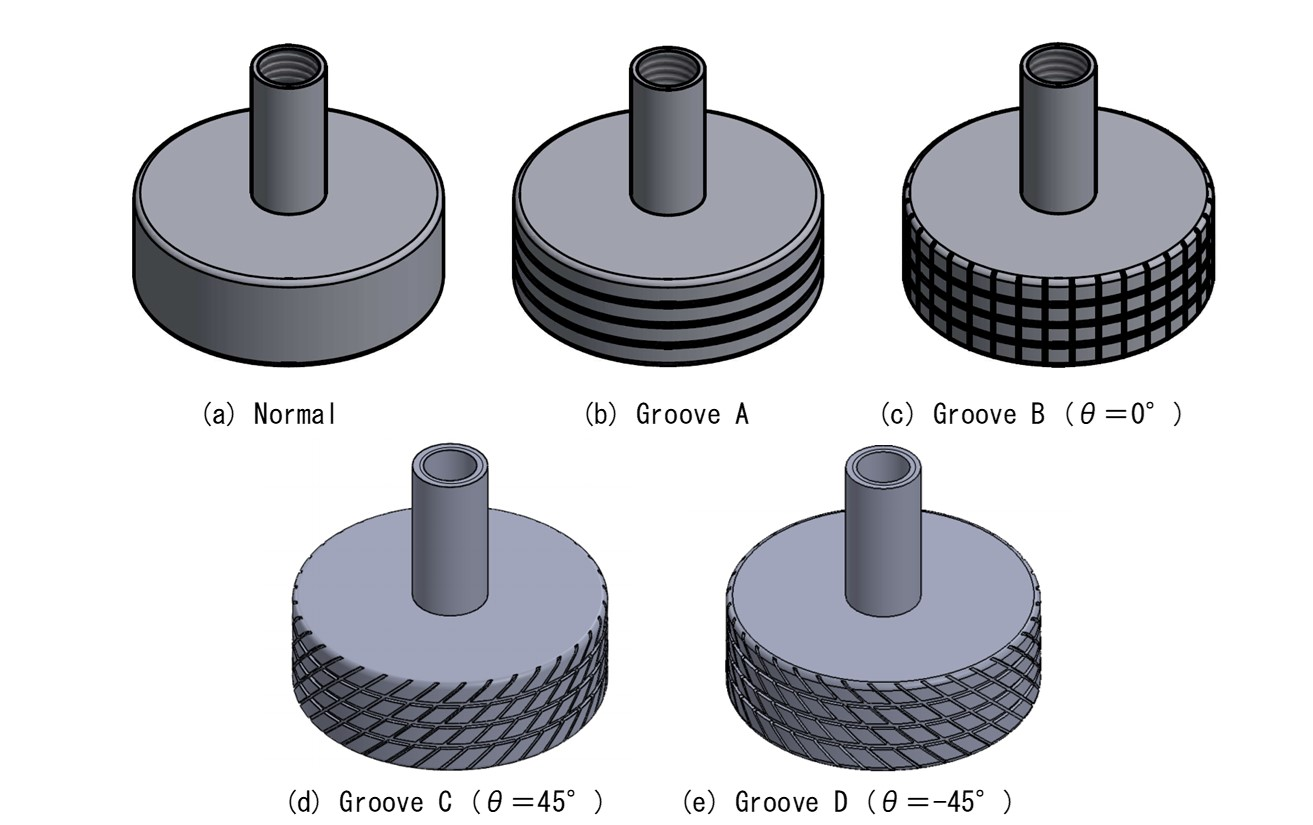
\includegraphics[width=70mm]{images/models_1.jpg}
        \caption{Image of models}
        ※ Type a, Type b,Type b は省略
    \end{center}
\end{figure}
\subsection{測定結果}
データの処理ができていないため、
例として Normal の抗力の実験結果 (実験2回目) のグラフを示す.
\begin{figure}[htbp]
    \begin{center}
        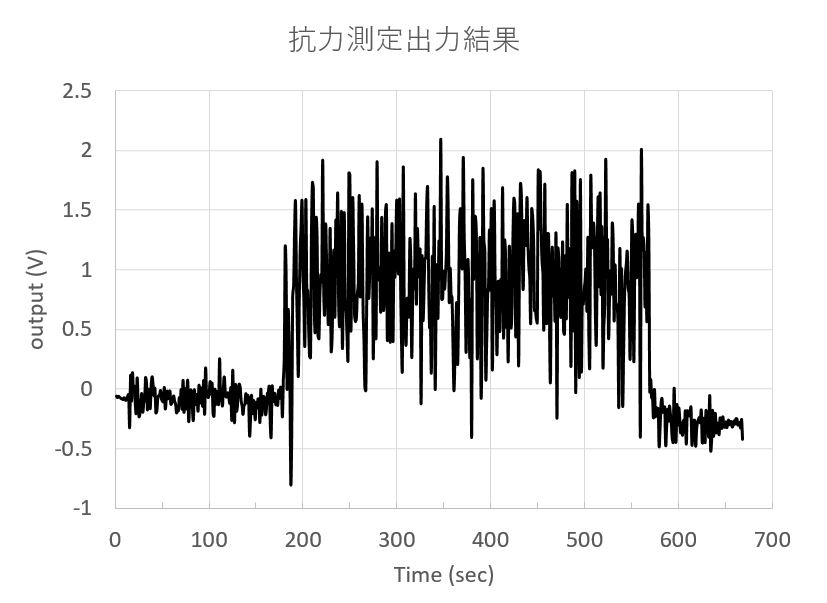
\includegraphics[width=80mm]{images/graph.jpg}
        \caption{Result of Normal's drag}
    \end{center}
\end{figure}
\newpage
\subsection{今後の研究方針}
\begin{itemize}
    \item [$\blacksquare$] \textgt{ノイズの除去}\\
    それぞれのモデルにおける作用力の違いを明らかにするため、
    まずは測定データのノイズを除去する必要がある。
    したがって、FFTの理解及びプログラムへ実装し、不要な周波数成分の除去を行う.
    \item [$\blacksquare$] \textgt{ドリフトの考慮}\\
    測定開始から時間経過とともに基準点が変動していくドリフトを考慮する必要がある。
    そのため、その方法を検討・試行して、実用的なデータを得られるようにする。
    \item [$\blacksquare$] \textgt{校正実験データの適用}\\
    6月に行ったひずみゲージの校正実験結果をもとに
    出力電圧を作用力へと換算し、モデルごとの差異を確かめる。
\end{itemize}
\section{今月の予定}
\begin{itemize}
    \item [$\blacksquare$] \textgt{FFTの実装}
    \begin{itemize}
        \item [$\bullet$] FFTのプログラムの作成
        \item [$\bullet$] バンドパスフィルタの適切な設定
        \item [$\bullet$] 9月下旬を目標
    \end{itemize}
    \item [$\blacksquare$] \textgt{ドリフト補正方法の検討}
    \begin{itemize}
        \item [$\bullet$] 情報収集
        \item [$\bullet$] 補正方法の試行
        \item [$\bullet$] 10月度報告会を目標
    \end{itemize}
\end{itemize}

\section{参考文献}
\end{document}